
\chapter[Dao động cơ, dao động tuần hoàn, dao động điều hòa;\\
Dạng bài: Phương trình dao động điều hòa]{Dao động cơ, dao động tuần hoàn, dao động điều hòa;\\Dạng bài: Phương trình dao động điều hòa}
\section{Lý thuyết}
\subsection{Dao động cơ}
Dao động cơ là chuyển động qua lại của một vật quanh một vị trí cân bằng.

Dao động cơ có thể là tuần hoàn hoặc không tuần hoàn.
\begin{center}
	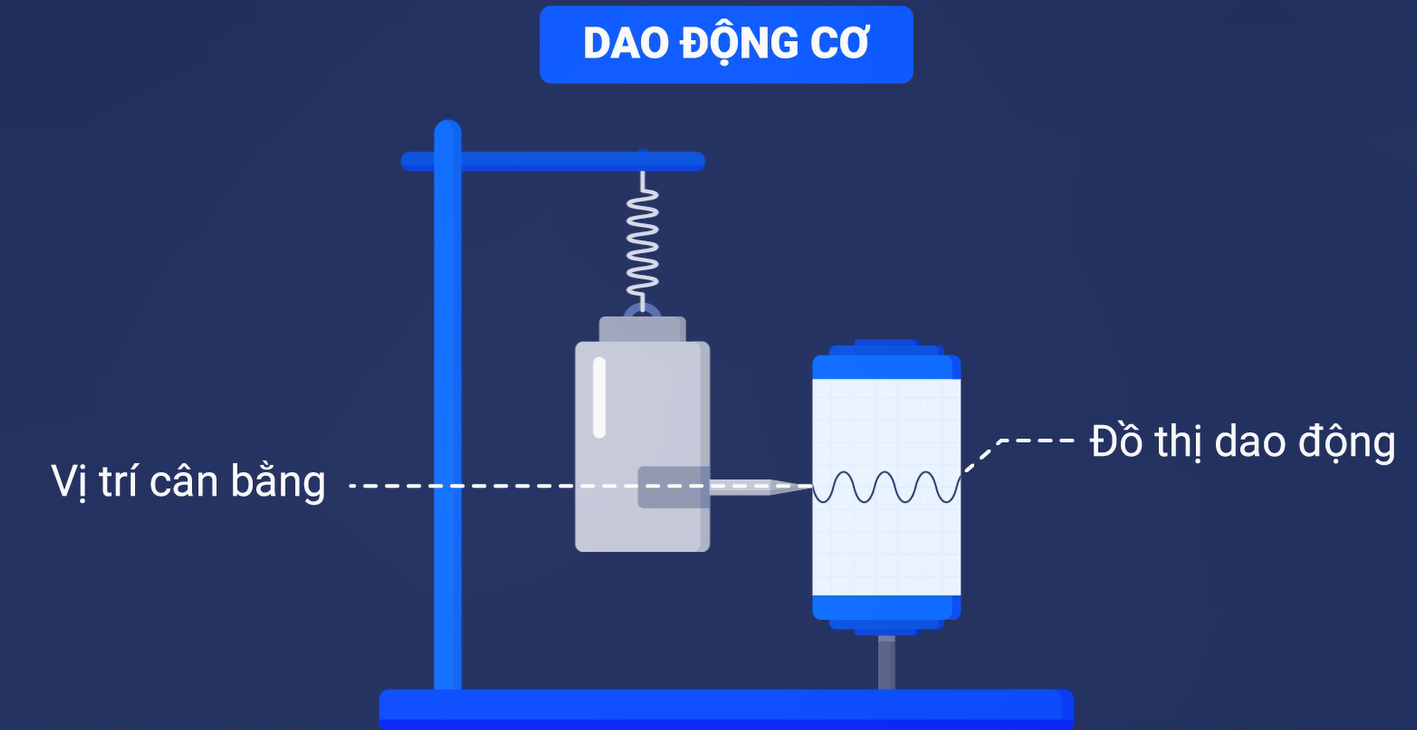
\includegraphics[scale=0.35]{../figs/VN12-PH-02-L-001-1-V2-1}
\end{center}
\subsection{Dao động tuần hoàn}
Dao động tuần hoàn là dao động mà sau những khoảng thời gian bằng nhau, vật trở lại về vị trí cũ và chiều chuyển động theo hướng cũ (trở lại trạng thái ban đầu).
\subsection{Dao động điều hòa}
Dao động điều hòa là dao động trong đó li độ của vật là một hàm cosin (hay sin) của thời gian.
\begin{center}
	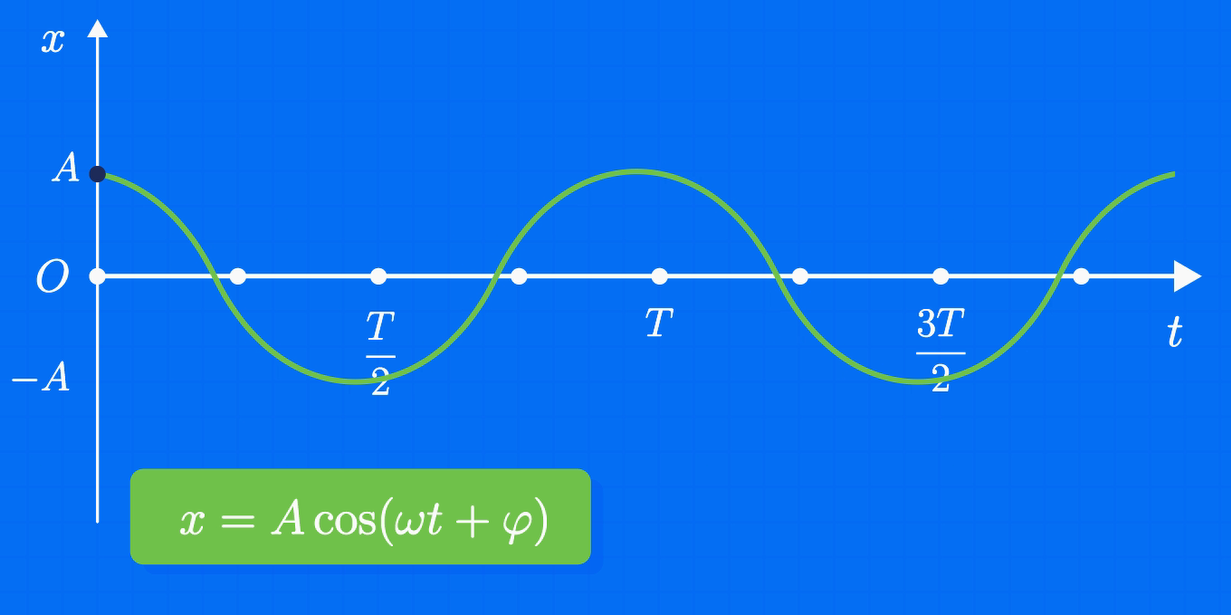
\includegraphics[scale=0.4]{../figs/VN12-PH-02-L-001-1-V2-2}
\end{center}
\luuy{Dao động điều hòa thì chắc chắn là dao động tuần hoàn, nhưng dao động tuần hoàn chưa chắc là dao động điều hòa.}
\subsection{Phương trình dao động điều hòa}
Phương trình dao động điều hòa:
\begin{equation*}
	x=A\cos\left(\omega t+\varphi\right)
\end{equation*}
\begin{center}
	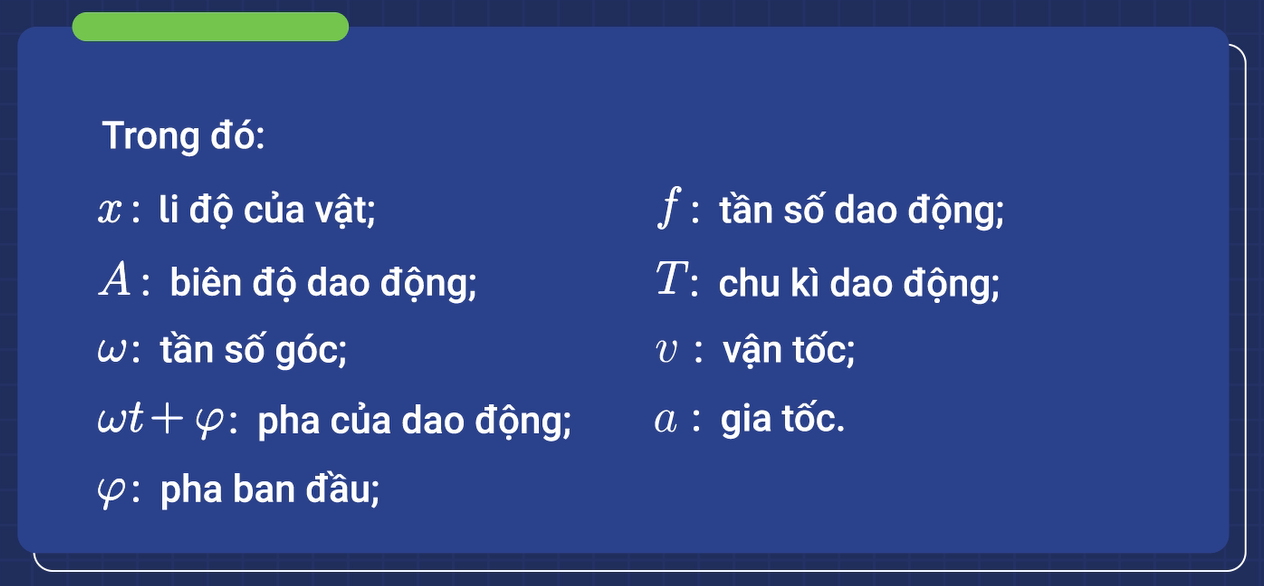
\includegraphics[scale=0.4]{../figs/VN12-PH-02-A-001-1-V2-1.png}
\end{center}
\luuy{
	Đôi khi dao động điều hòa còn được biểu diễn bởi phương trình:
	\begin{equation*}
		x=x_0+A\cos\left(\omega t+\varphi\right);
	\end{equation*}
	với $x_0$ là tọa độ vị trí cân bằng ($x_0$ là hằng số).
}
\subsection{Chu kì, tần số, tần số góc của dao động điều hòa}
\subsubsection{Chu kì}
Chu kì là khoảng thời gian để vật thực hiện \bltext{một dao động toàn phần}, kí hiệu: $T$.
\subsubsection{Tần số}
Tần số là số dao động toàn phần thực hiện được trong \bltext{một giây}, kí hiệu: $f$, đơn vị: Hz.
\subsubsection{Tần số góc}
Tần số góc là tốc độ biến đổi của góc pha, kí hiệu: $\omega$, đơn vị: rad/s.
\subsubsection{Công thức liên hệ giữa chu kì, tần số, tần số góc}
\begin{equation*} \omega = \dfrac{2\pi}{T} = 2\pi f. \end{equation*}
\begin{center}
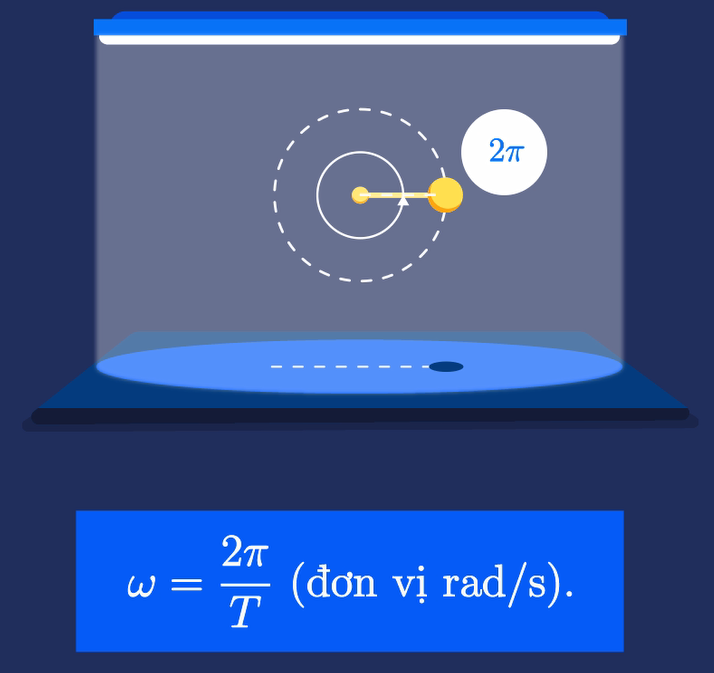
\includegraphics[scale=0.5]{../figs/VN12-PH-02-A-001-1-V2-2.png}
\end{center}
\section{Mục tiêu bài học - Ví dụ minh họa}
\begin{dang}{Ghi nhớ được định nghĩa\\ dao động cơ, dao động tuần hoàn,\\ dao động điều hòa}
	\viduii{1}{Dao động cơ học là
		\begin{mcq}(1)
			\item chuyển động tuần hoàn quanh một vị trí cân bằng.
			\item chuyển động lặp đi lặp lại nhiều lần quanh vị trí cân bằng. 
			\item chuyển động đung đưa nhiều lần quanh vị trí cân bằng.
			\item chuyển động thẳng biến đổi quanh một vị trí cân bằng. 
		\end{mcq}
	}
	{\begin{center}
			\textbf{Hướng dẫn giải}
		\end{center}
		
		Dao động cơ học là chuyển động lặp đi lặp lại nhiều lần quanh vị trí cân bằng.
		
		\textbf{Đáp án: B.}
	}
	\viduii{1}{Dao động điều hòa có đặc điểm:
		\begin{mcq}
			\item li độ của vật biến thiên theo thời gian.
			\item gia tốc của vật là một hàm cosin (hay sin) của thời gian.
			\item vận tốc của vật là một hàm cosin (hay sin) của thời gian.
			\item li độ của vật là một hàm cosin (hay sin) của thời gian.
		\end{mcq}
	}
	{\begin{center}
			\textbf{Hướng dẫn giải}
		\end{center}
		
		Dao động điều hòa là dao động trong đó li độ của vật là một hàm cosin (hay sin) của thời gian.
		
		\textbf{Đáp án: D.}
	}
	
\end{dang}
\begin{dang}{Nhận biết được dao động cơ,\\ dao động tuần hoàn, dao động điều hòa}
	\viduii{2}{Dao động nào sau đây \textbf{không} phải là dao động tuần hoàn?
		\begin{mcq}
			\item Dao động của con lắc trong chiếc đồng hồ quả lắc chạy đúng giờ.
			\item Dao động của chiếc thuyền nhấp nhô trên biển.
			\item Dao động của con lắc đơn khi chỉ có trọng lực tác dụng.
			\item Dao động điều hòa của một vật bất kì.
		\end{mcq}
		
	}
	{\begin{center}
			\textbf{Hướng dẫn giải}
		\end{center}
		
		Dao động của chiếc thuyền nhấp nhô trên biển không phải là dao động tuần hoàn vì sau những khoảng thời gian bằng nhau, vật không trở lại trạng thái ban đầu.
		
		\textbf{Đáp án: B.}
	}
	\viduii{2}{Kết luận nào dưới đây là đúng?
		\begin{mcq}
			\item Dao động điều hòa thì chắc chắn là dao động tuần hoàn.
			\item Dao động cơ chắc chắn là dao động tuần hoàn.
			\item Dao động tuần hoàn thì chắc chắn là dao động điều hòa.
			\item Dao động điều hòa không phải là dao động cơ.
		\end{mcq}
	}
	{\begin{center}
			\textbf{Hướng dẫn giải}
		\end{center}
		
		Dao động điều hòa thì chắc chắn là dao động tuần hoàn, nhưng dao động tuần hoàn chưa chắc là dao động điều hòa
		
		\textbf{Đáp án: A.}
	}
\end{dang}
\begin{dang}{Giải thích được các đại lượng có trong phương trình dao động điều hòa}
	\ppgiai{So sánh phương trình đã cho và phương trình dao động điều hòa tổng quát để xác định đại lượng mà đề bài đã hỏi.}
	\viduii{2}{Một vật dao động điều hòa theo phương trình $x=A \cos (2\omega t + \varphi)$. Tần số góc của dao động là
		\begin{mcq}(4)
			\item $\omega t$.
			\item $\omega$.
			\item $2 \omega$.
			\item $2\omega t + \varphi$.
		\end{mcq}
	}
	{\begin{center}
			\textbf{Hướng dẫn giải}
		\end{center}
		
		Vật dao động theo phương trình $x=A \cos (2\omega t + \varphi)$, do đó tần số góc là $2\omega$.
		
		\textbf{Đáp án: C.}
	}
	\viduii{2}{Phát biểu nào dưới đây là đúng khi so sánh giữa pha và pha ban đầu của một vật dao động điều hòa?
		\begin{mcq}
			\item Pha ban đầu chính là pha của dao động ở thời điểm ban đầu.
			\item Pha ban đầu chính là pha ở thời điểm bất kì của dao động.
			\item Pha ban đầu và pha có đơn vị khác nhau.
			\item Pha ban đầu luôn luôn bằng 0, còn pha thì có thể khác 0.
		\end{mcq}
	}
	{\begin{center}
			\textbf{Hướng dẫn giải}
		\end{center}
		
		Pha ban đầu chính là pha của dao động ở thời điểm ban đầu (khi $t=0$).
		
		\textbf{Đáp án: A.}
	}
	
\end{dang}
\begin{dang}{Sử dụng được phương trình dao động điều hòa để xác định giá trị tức thời của li độ}
	\viduii{2}{Một vật dao động điều hòa với phương trình $x=4 \cos (10\pi t + \pi /3 )\ \text{(cm)}$. Ở thời điểm ban đầu, vật có li độ là
		\begin{mcq}(4)
			\item $x=4\ \text{cm}$.
			\item $x=3\ \text{cm}$.
			\item $x=2\ \text{cm}$.
			\item $x=1\ \text{cm}$.		\end{mcq}
		
	}
	{\begin{center}
			\textbf{Hướng dẫn giải}
		\end{center}
		
		Ở thời điểm ban đầu ($t=0$) thì $x=4\cos(0+\pi / 3) = 4 \cos (\pi / 3) = 2\ \text{cm}$.
		
		\textbf{Đáp án: C.}
	}
	
	\viduii{2}{Một vật dao động điều hòa dọc theo trục O$x$ với phương trình $x=A\cos(\pi t)\ \text{(cm)}$. Nếu chọn gốc tọa độ O tại vị trí cân bằng của vật thì gốc thời gian $t=0$ là lúc vật
		\begin{mcq}
			\item ở vị trí li độ cực đại ở phần dương của trục O$x$.
			\item qua vị trí cân bằng ngược chiều dương của trục O$x$.
			\item ở vị trí li độ cực đại ở phần âm của trục O$x$.
			\item qua vị trí cân bằng cùng chiều dương của trục O$x$.
		\end{mcq}
		
	}
	{\begin{center}
			\textbf{Hướng dẫn giải}
		\end{center}
		
		Ở thời điểm $t=0$ thì $x=A \cos(0)=A$.
		
		Vậy vật ở vị trí li độ cực đại ở phần dương của trục O$x$.
		
		\textbf{Đáp án: A.}
	}
\end{dang}
\begin{dang}{Xây dựng được phương trình dao động điều hòa}
	\ppgiai{
		\subsubsection{Phương pháp đại số}
		
		Phương trình dao động điều hòa có dạng:
		\begin{equation*}
			x=A\cos\left(\omega t+\varphi\right).
		\end{equation*}
		Trong phương trình dao động điều hòa, biên độ $A$, tần số góc $\omega$ và pha ban đầu $\varphi$ là những đại lượng hằng số. Do đó, để viết phương trình dao động điều hòa ta cần xác định biên độ $A$, tần số góc $\omega$ và pha ban đầu $\varphi$.
		\begin{description}
			\item[Bước 1:] Xác định biên độ $A$
			
			Biên độ $A$ có thể được xác định bằng các công thức sau:
			\begin{itemize}
				\item Công thức độc lập với thời gian:
				\begin{equation*}
					x^2+\dfrac{v^2}{\omega^2}=A^2 \Rightarrow A=\sqrt{x^2+\dfrac{v^2}{\omega^2}},
				\end{equation*}
				hay
				\begin{equation*}
					v^2+\dfrac{a^2}{\omega^2}=\omega^2 A^2 \Rightarrow A=\sqrt{\dfrac{v^2}{\omega^2}+\dfrac{a^2}{\omega^4}};
				\end{equation*}
				\item Công thức giá trị lớn nhất của vận tốc và gia tốc:
				\begin{equation*}
					v_\text{max}=\omega A\Rightarrow A=\dfrac{v_\text{max}}{\omega},
				\end{equation*}
				hay
				\begin{equation*}
					a_\text{max}=\omega^2 A\Rightarrow A=\dfrac{a_\text{max}}{\omega^2},
				\end{equation*}
				hay
				\begin{equation*}
					A=\dfrac{v_\text{max}^2}{a_\text{max}};
				\end{equation*}
				\item Công thức độ dài quỹ đạo $L$ và quãng đường $S$ đi trong một chu kì
				\begin{equation*}
					A=\dfrac{L}{2}=\dfrac{S}{4}.
				\end{equation*}
			\end{itemize}
			\item[Bước 2:] Xác định tần số góc $\omega$
			
			Tần số góc $\omega$ có thể được xác định bằng các công thức sau:
			\begin{itemize}
				\item Công thức liên hệ giữa tần số góc $\omega$, chu kì $T$ và tần số $f$:
				\begin{equation*}
					\omega=2\pi f=\dfrac{2\pi}{T};
				\end{equation*}
				\item Công thức giá trị lớn nhất của vận tốc và gia tốc:
				\begin{equation*}
					v_\text{max}=\omega A\Rightarrow \omega=\dfrac{v_\text{max}}{A},
				\end{equation*}
				hay
				\begin{equation*}
					a_\text{max}=\omega^2 A\Rightarrow \omega=\sqrt{\dfrac{a_\text{max}}{A}},
				\end{equation*}
				hay
				\begin{equation*}
					a_\text{max}=\omega v_\text{max}\Rightarrow \omega=\dfrac{a_\text{max}}{v_\text{max}};
				\end{equation*}
				\item Công thức độc lập thời gian:
				\begin{equation*}
					x^2+\dfrac{v^2}{\omega^2}=A^2 \Rightarrow \omega=\sqrt{\dfrac{v^2}{A^2-x^2}}.
				\end{equation*}
			\end{itemize}
			\item[Bước 3:] Xác định pha ban đầu $\varphi$
			
			Pha ban đầu $\varphi$ có thể được xác định dựa vào thời điểm ban đầu $t_0=0$:
			\begin{equation*}
				\left\{
				\begin{matrix}
					x_0=A\cos\varphi\\
					v_0=-\omega A\sin\varphi
				\end{matrix}
				\right.
				\Rightarrow
				\left\{
				\begin{matrix}
					\cos\varphi=\frac{x_0}{A}\\
					\sin\varphi=-\frac{v}{\omega A}.
				\end{matrix}
				\right.
			\end{equation*}
			Từ $\cos\varphi$ và $\sin\varphi$ ta tìm được 2 giá trị của $\varphi$ rồi dựa vào điều kiện ban đầu của đề bài là vật đi cùng chiều dương hay ngược chiều dương để loại đi một giá trị.
			\begin{itemize}
				\item $\varphi>0$ nếu vật đi ngược chiều dương;
				\item $\varphi<0$ nếu vật đi theo chiều dương;
			\end{itemize}
		\end{description}
		
		\subsubsection{Phương pháp sử dụng đường tròn lượng giác}
		
		Phương pháp đường tròn lượng giác được sử dụng để xác định pha ban đầu $\varphi$. Biên độ $A$ và tần số góc $\omega$, được xác định dựa vào phương pháp đại số. 
		\begin{description}
			\item[Bước 1:] Vẽ trục $\text{O}x$ gắn vào đường tròn bán kính $R=A$.
			\item[Bước 2:] Xác định vị trí $x_0$ trên đường tròn lượng giác và chiều của chuyển động. Quy ước rằng chiều dương là chiều ngược chiều kim đồng hồ.
			\item[Bước 3:] Xác định pha ban đầu.
			\begin{center}
				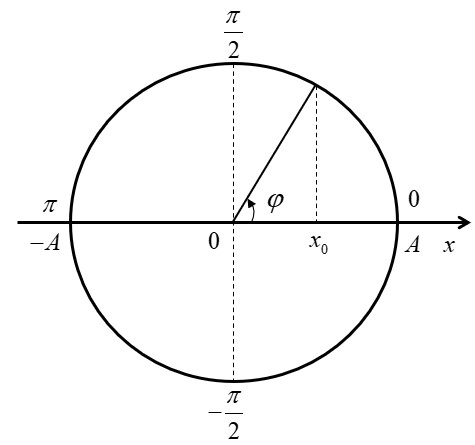
\includegraphics[scale=0.7]{../figs/VN12-PH-02-A-001-1-V2-3.jpg}
			\end{center}
		\end{description}
		\manatip{Một số giá trị cung lượng giác đặc biệt:
			\begin{center}
				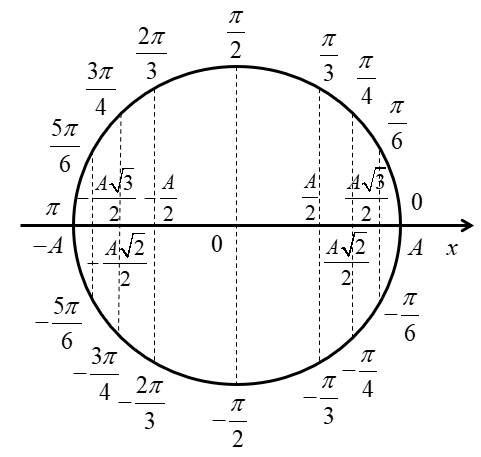
\includegraphics[scale=0.7]{../figs/VN12-PH-02-A-001-1-V2-4.jpg}
			\end{center}
		}
		
		\subsubsection{Phương pháp số phức}
		Phương trình tổng quát của dao động điều hòa có thể viết dưới dạng số phức như sau:
		\begin{equation*}
			x_0-\dfrac{v_0}{\omega}\cdot i=A\angle\varphi;
		\end{equation*}
		trong đó:
		\begin{itemize}
			\item $x_0$ là li độ của vật tại thời điểm ban đầu;
			\item $v_0$ là vận tốc của vật tại thời điểm ban đầu;
			\item $i$ là phần ảo của số phức.
		\end{itemize}
		
		Ở phương pháp này ta tính tần số góc $\omega$ như phương pháp đại số. Sau đó bấm máy tính chuyển từ số phức dạng Descartes sang dạng lượng giác để xác định biên độ $A$ và pha ban đầu $\varphi$.
		
		Gợi ý cách bấm máy tính Casio fx-580VN X:
		\begin{itemize}
			\item Thiết lập môi trường tính toán số phức với lệnh:
			\begin{center}
				
\includegraphics[scale=0.5]{../figs/VN12-PH-02-A-001-1-V2-5.jpg}
			\end{center}
			\item Nhập số phức cần chuyển đổi từ dạng Descartes sang dạng lượng giác
			\item Thực hiện chuyển đổi số phức bằng lệnh:
			\begin{center}
				
\includegraphics[scale=0.5]{../figs/VN12-PH-02-A-001-1-V2-6.jpg}
			\end{center}
			\item Cài đặt đơn vị góc ở radian (nếu cần):
			\begin{center}
				
\includegraphics[scale=0.5]{../figs/VN12-PH-02-A-001-1-V2-7.jpg}
			\end{center}
		\end{itemize}	
	}
	\viduii{3}{Trong các phương trình sau, phương trình nào \textbf{không} biểu thị dao động điều hòa?
		\begin{mcq}(2)
			\item $x=5\cos \pi t + 1\ \text{cm}$.
			\item $x = 3t \cos \left(100\pi t + \dfrac{\pi}{6}\right)\ \text{cm}$. 
			\item $x=2\sin^2 \left(2\pi t +\dfrac{\pi}{6}\right)\ \text{cm}$.
			\item $x=3\sin 5\pi t + 3\cos 5\pi t\ \text{cm}$. 
		\end{mcq}
		
	}
	{\begin{center}
			\textbf{Hướng dẫn giải}
		\end{center}
		
		$x=5\cos \pi t + 1\ \text{cm}$ là hàm điều hòa, với $x_0 =\SI{1}{cm}$ là tọa độ ban đầu.
		
		$x=3\sin 5\pi t + 3\cos 5\pi t\ \text{cm} = 3\sqrt 2 \cos \left(5\pi t -\dfrac{\pi}{4}\right)\ \text{cm}$ là một hàm điều hoà.
		
		$x=2\sin^2 \left(2\pi t +\dfrac{\pi}{6}\right)\ \text{cm} = 1+ \cos \left(4\pi t +\dfrac{\pi}{3}\right)\ \text{cm}$ là một hàm điều hòa.
		
		\textbf{Đáp án: B.}
	}
	\viduii{3}{Một chất điểm dao động điều hòa trên trục $\text{O}x$ với chu kì $\SI{0,2}{\second}$. Lấy gốc thời gian là lúc chất điểm đi qua vị trí có li độ $\SI{2}{\centi\meter}$ ngược chiều dương với tốc độ $20\pi\, \text{cm/s}$. Phương trình dao động của chất điểm là
		\begin{mcq}(2)
			\item $x=2\sqrt{2}\cos\left(10\pi t+\dfrac{\pi }{4} \right)\,\text{cm}$.
			\item $x=2\sqrt{2}\cos \left(10\pi t-\dfrac{\pi }{4} \right)\,\text{cm}$.
			\item $x=2\sqrt{2}\cos \left(10\pi t+\dfrac{3\pi }{4} \right)\,\text{cm}$.
			\item $x=2\sqrt{2}\cos \left(10\pi t+\dfrac{3\pi }{4} \right)\,\text{cm}$.
		\end{mcq}
	}
	{\begin{center}
			\textbf{Hướng dẫn giải}
		\end{center}
		
		\subsubsection{Phương pháp đại số}
		
		Xác định tần số góc $\omega$
		
		\begin{equation*}
			\omega =\frac{2\pi }{T}=\frac{2\pi }{\SI{0,2}{\second}}=10\pi \,\text{rad/s}.
		\end{equation*}
		
		Xác định biên độ $A$
		
		Gốc thời gian là lúc chất điểm đi qua vị trí có li độ $\SI{0,2}{\centi\meter}$ ngược chiều dương với tốc độ $20\pi\, \text{cm/s}$ nên $x_0=\SI{2}{\centi\meter}$ và $v_0=-20\pi\, \text{cm/s}$.
		
		Áp dụng công thức độc lập thời gian
		\begin{equation*}
			A=\sqrt{x^2+\dfrac{v^2}{\omega ^2}}=\sqrt{(\SI{2}{\centi\meter})^2+\dfrac{(-20\pi\, \text{cm/s} )^2}{(10\pi \,\text{rad/s} )^2}}=2\sqrt{2}\,\text{cm}.
		\end{equation*}
		
		Xác định pha ban đầu $\varphi$
		
		\begin{equation*}
			\cos\varphi =\dfrac{x_{0}}{A}=\frac{1}{\sqrt{2}}\Rightarrow\varphi =\pm\dfrac{\pi }{4}
		\end{equation*}
		
		Vì tại thời điểm $t=0$ chất điểm đi theo chiều âm nên loại $\varphi =-\dfrac{\pi }{4}$.
		
		Do đó, $\varphi =\dfrac{\pi }{4}$.
		
		Vậy phương trình dao động của chất điểm là
		\begin{equation*}
			x=2\sqrt{2}\cos\left(10\pi t+\dfrac{\pi }{4} \right)\,\text{cm}.
		\end{equation*}
		
		\subsubsection{Phương pháp sử dụng đường tròn lượng giác}
		
		Tần số góc $\omega$ của dao động là
		
		\begin{equation*}
			\omega =\frac{2\pi }{T}=\frac{2\pi }{\SI{0,2}{\second}}=10\pi \,\text{rad/s}.
		\end{equation*}
		
		Gốc thời gian là lúc chất điểm đi qua vị trí có li độ $\SI{0,2}{\centi\meter}$ ngược chiều dương với tốc độ $20\pi\, \text{cm/s}$ nên $x_0=\SI{2}{\centi\meter}$ và $v_0=-20\pi\, \text{cm/s}$.
		
		Áp dụng công thức độc lập thời gian ta xác định được biên độ $A$ của dao động là
		\begin{equation*}
			A=\sqrt{x^2+\dfrac{v^2}{\omega ^2}}=\sqrt{(\SI{0,2}{\centi\meter})^2+\dfrac{(-20\pi\, \text{cm/s} )^2}{(10\pi \,\text{rad/s} )^2}}=2\sqrt{2}\,\text{cm}.
		\end{equation*}
		
		Vì $x_0=\SI{0,2}{\centi\meter}=\dfrac{A\sqrt{2}}{2}$ nên $\varphi =\pm\dfrac{\pi }{4}$.
		
		Mà tại thời điểm ban đầu vật đi ngược chiều dương nên $\varphi =\dfrac{\pi }{4}$.
		
		\begin{center}
			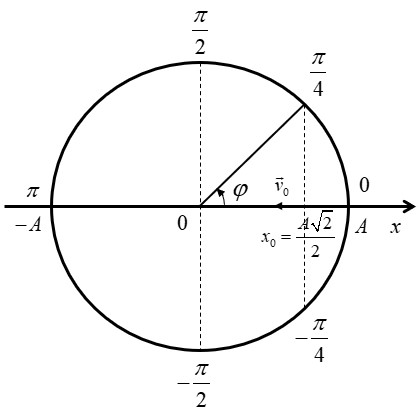
\includegraphics[scale=0.8]{../figs/VN12-PH-02-A-001-1-V2-8.jpg}
		\end{center}
		
		Vậy phương trình dao động của chất điểm là
		\begin{equation*}
			x=2\sqrt{2}\cos\left(10\pi t+\dfrac{\pi}{4} \right)\,\text{cm}.
		\end{equation*}
		
		\subsubsection{Phương pháp số phức (giải bằng máy tính)}
		
		Tần số góc $\omega$ của dao động là
		
		\begin{equation*}
			\omega =\frac{2\pi }{T}=\frac{2\pi }{\SI{0,2}{\second}}=10\pi \,\text{rad/s}.
		\end{equation*}
		
		Phương trình dao động điều hòa của vật có thể viết dưới dạng số phức như sau
		\begin{equation*}
			2-\dfrac{-20\pi}{10\pi}\cdot i=2+2i.
		\end{equation*}
		
		Sử dụng máy tính Casio fx-580VN X chuyển đổi số phức từ dạng Descartes sang dạng lượng giác
		\begin{center}
			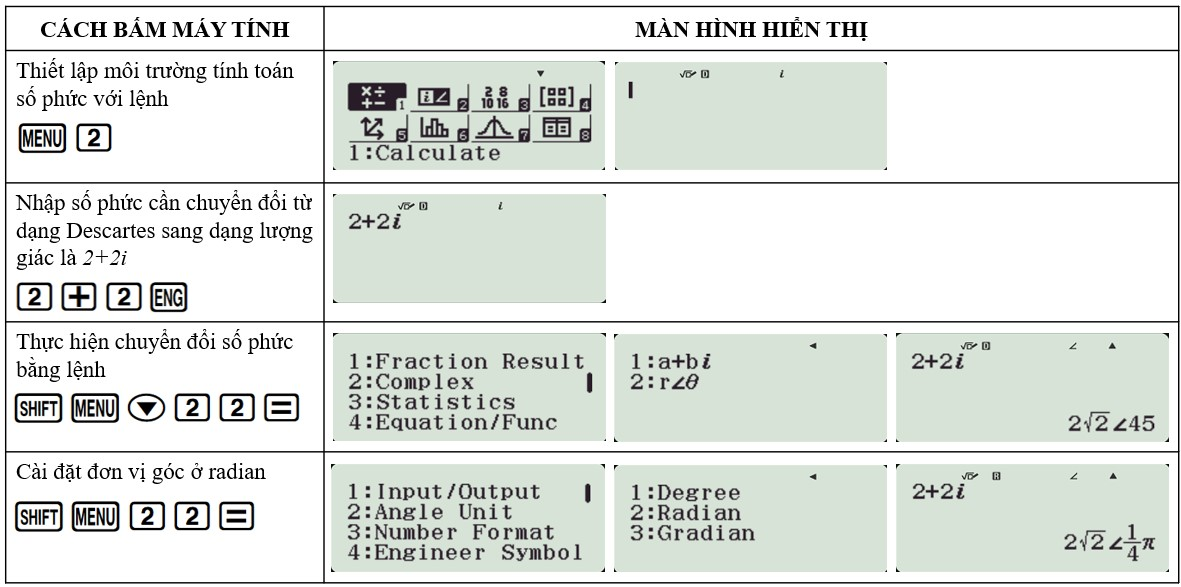
\includegraphics[scale=0.54]{../figs/VN12-PH-02-A-001-1-V2-9.jpg}
		\end{center}
		
		
		
		Kết quả là
		\begin{equation*}
			2+2i=2\sqrt{2}\angle\dfrac{\pi}{4}.
		\end{equation*}
		
		Vậy phương trình dao động của chất điểm là
		\begin{equation*}
			x=2\sqrt{2}\cos\left(10\pi t+\dfrac{\pi}{4} \right)\,\text{cm}.
		\end{equation*}
		
		\textbf{Đáp án: A.}
	}
\end{dang}
